\documentclass[journal=jcisd8,manuscript=article,layout=twocolumn]{achemso}
\usepackage{amsmath}
\usepackage{amssymb}
%\usepackage{widetext}
\usepackage{verbatim}
\usepackage{graphicx}
% \usepackage{multicol}
\usepackage[normalem]{ulem} % for strikethrough
\usepackage[obeyFinal]{easy-todo}
\usepackage{dutchcal}
\usepackage{xfrac}
\usepackage{footmisc}

\newcommand{\figurewidth}{.48\textwidth}
\renewcommand{\epsilon}{\varepsilon}
\newcommand{\dz}{\,\mathrm{d}z}
\graphicspath{{Figures/}}
\newcommand{\onlinecite}[1]{\hspace{-1 ex} \nocite{#1}\citenum{#1}}
\SectionNumbersOn
%\DeclareUnicodeCharacter{2009}{FIXME}

\author{Hanne S. Antila}
\affiliation{Department of Theory and Bio-Systems, Max Planck Institute of Colloids and Interfaces, 14424 Potsdam, Germany}
\email{hanne.antila@mpikg.mpg.de}

\author{Tiago M. Ferreira}
\affiliation{NMR Group --- Institute for Physics, Martin-Luther University Halle--Wittenberg, 06120 Halle (Saale), Germany}

\author{O. H. Samuli Ollila}
\affiliation{Institute of Biotechnology, University of Helsinki, 00014 Helsinki, Finland}

\author{Markus S. Miettinen}
\affiliation{Department of Theory and Bio-Systems, Max Planck Institute of Colloids and Interfaces, 14424 Potsdam, Germany}
\email{markus.miettinen@iki.fi}

%\title{Using open data to benchmark internal dynamics of phosphatidylcholine in molecular dynamics simulations}
\title{Using open data to rapidly bench\-mark bio\-molecular simulations: Phospholipid conformational dynamics}
%\title{Using open data to rapidly bench\-mark simulations of unstructured biomolecules}
%\title{Using open data to rapidly bench\-mark internal dynamics of unstructured biomolecules in molecular dynamics simulations}
\begin{document}


\begin{abstract}
Molecular dynamics (MD) simulations are widely used to
    study the atomistic structure and dynamics of biomembranes. It
    remains unknown, however, how well the conformational dynamics
    observed in MD simulations correspond to those occurring in real
    life phospholipids. The accuracy of such time scales in MD can be
    assessed by comparing against the effective correlation times $\tau_\mathrm e$ of
    the C-H bonds measured in nuclear magnetic resonance experiments
    (J. Chem. Phys. 142 044905 (2015)).

Here, we
use a large set of open data trajectories made public by the NMRlipids project (\url{ nmrlipids.blogspot.fi}) to
perform an unprecedented test on
the conformational dynamics of phospholipids as
produced by several commonly used MD models (force fields).
We find that
none of the tested force fields to reproduce all the effective correlation times within experimental error, much like they do
not provide accurate conformational ensembles (J. Phys. Chem. B 119 15075 (2015)). However, the dynamics observed in CHARMM36 and Slipids were more realistic than those seen in the Amber Lipid14, OPLS-based MacRog, and
 GROMOS-based Berger force fields, where dynamics of the glycerol backbone was unrealistically slow. \todo{Tiago: We need a punchline highlighting that the results and findings obtained are extremely important for the lipid MD simulation community and that they were only possible due to the open data}

\end{abstract}

\section{Introduction}
Ever since the conception of Protein Data Bank (PDB)~\cite{nnb1971,wwPDB2019} and GenBank~\cite{jordan1982,sayers2020},
open access to standardised and searchable pools of experimental data has
%shaped the state of the art of 
revolutionized
scientific
research. %in life sciences.
Constantly growing and improving in fidelity
%as well as identifying~\cite{hobohm1992,levitt2007} and filling~\cite{meszaros2019} gaps in the databanks themselves
due to collaborative effort~\cite{levitt2007,Brzezinski:2020a,Harris:2003a,Steinegger:2020a}, %For IDPs:Necci:2020a?
%Wlodawer:2020a
the now hundreds of databanks~\cite{Rigden:2020a}
%The entirely new way of doing science of bio- and cheminformatics
fuel the data-driven development of
biomolecular structure determination~\cite{Simpkin:2019a},
refinement~\cite{Leelananda:2020a}, %{DiMaio:2015a}
prediction~\cite{Senior:2020a}, and
design~\cite{huang2016} approaches,
%characterisation \cite{burley2018}, (such as molecular replacement~\cite{rossmann62} in macromolecular x-ray crystallography and 3D electron microscopy)
as well as development of
drugs~\cite{Westbrook:2019a,Martinez-Mayorga:2020a}, %kirchmair08
materials~\cite{Senderowitz:2018a,Wan:2019a},
and more~\cite{Perez-Riverol:2019a,Feng:2020a}.
It is clear that open data enables scientific
progress that is far beyond the resources of a single research group or institute.
%
Consequently,
the call for public availability and conservation of data has extended to molecular dynamics (MD) simulation trajectories of biomolecules~\cite{Feig:1999a,Tai:2004a,Silva:2006a}, and the discussion on how and by whom such databanks for dynamic structures would be set up is currently active~\cite{Hildebrand:2019a,Abraham:2019a,Abriata:2020a,Hospital:2020a}.
%
While no general MD trajectory databank %, accepting submissions of MD trajectories of any type of biomolecular system,
currently operates,
individual databanks are accepting contributions on
nucleic acid~\cite{Hospital:2016a}, %BIGNASim
protein/DNA/RNA~\cite{Bekker:2020a}, %BSM-Arc
cyclodextrin~\cite{Mixcoha:2016a}, %Cyclo-lib
G-protein-coupled receptor~\cite{Rodriguez-Espigares:2019a}, %GPCRmd
and lipid bilayer~\cite{Miettinen:2019c} %NMRlipids Databank
simulations.

Since 2013, the NRMlipids Project (\url{nmrlipids.blogspot.fi}) has
promoted a fully open collaboration approach, where
the whole scientific research process---from initial ideas and discussions to
analysis methods, data, and publications---is all the time publicly available~\cite{botan15}.
While its main focus has been on conformational ensembles
of different lipid headgroups and on ion binding to lipid membranes \cite{botan15,catte16,Antila:2019a},
the NMR\-lipids Project has also built a databank~\cite{Miettinen:2019c} (\url{zenodo.org/communities/nmrlipids}) containing hundreds
of atomistic MD trajectories of lipid bilayers and
%These data are also partially
indexed at \url{nmrlipids.fi}.

MD databanks are expected to be particularly relevant for disordered biomolecules, such as
biological lipids composing cellular membranes or intrinsically disordered proteins.
These, in contrast to folded proteins or DNA strands,
cannot be meaningfully described by the coordinates of a single structure alone.
%, in their biologically relevant state as the core components of the cell's membranes, are intrinsically unstructured.
Realistic MD simulations, however,
can provide the complete conformational ensemble and dynamics of such molecules, as well as
enable studies of their biological functions in complex biomolecular assemblies.
Unfortunately, the current MD force fields largely fail to capture the conformational ensembles of lipid headgroups and
disordered proteins \cite{botan15,Antila:2019a,robustelli18,henriques18,virtanen20}.
Therefore, before they can be used to draw conclusions,
the quality of MD simulations
%in databanks and other applications
must always be carefully assessed against structurally sensitive experiments.
For lipid bilayers, such evaluation is possible against NMR and scattering data~\cite{Ollila:2016a}.

Here, we demonstrate the use of a pre-existing, publicly available set of MD trajectories to
rapidly evaluate the fidelity of phospholipid conformational dynamics in state-of-the-art force fields.
The speed at which individual molecules sample their conformational ensemble
%against experimental data in different force fields with unprecedented extent. 
%Using this freely available resource we demonstrate here, for the first time, the viability of creating new scientific knowledge solely through analysis of pre-existing, open access MD simulation data.
is traditionally used to assess if a given MD simulation has converged.
Going beyond such practicalities,
realistic dynamics are particularly desired for the intuitive interpretation of NMR %or other
experiments sensitive to molecular motions~\cite{Antila:2020a},
as well as to understand the dynamics of biological processes where
molecular deformations play a rate-limiting role, such as membrane fusion~\cite{han17}.
%
%By analyzing a wide set of publicly available phosphatidylcholine (PC) lipid bilayer MD trajectories, we test whether different MD models (force fields) reproduce the experimentally observed internal dynamics of PC lipids, and investigate if the dynamics of various models share common features. Such features can be used to draw general conclusions on the system, to avoid potential pitfalls in future simulations of bilayers, and to suggest future directions for experimental research.  In addition to simulations of one component bilayers under standard conditions, we study the effects of varying hydration and cholesterol content
%
The here presented comprehensive comparison of dynamics between experiments and different MD models %for phosphatidylcholine lipids
at various biologically relevant compositions and conditions is thus likely to facilitate the development of increasingly realistic phospholipid force fields. 

%Our analysis of an extensive set of data from different models brings to light the complex dynamics of lipid in their biological relevant disordered state.
Above all, our results demonstrate the power of publicly available MD trajectories
in creating new knowledge at a lowered computational cost and high potential for automation.  
%the pre-existing, 
We believe that this paves the way for novel applications of MD trajectory
%publicly available MD simulations
databanks, as well as underlines their usefulness---not only for lipid membranes,
but for all biomolecular systems.

%we intentionally restrict ourselves to re-use existing, publicly available simulation trajectories. This is to demonstrate the power of open, well documented data in creating new knowledge at a lowered cost. The main source of data was the collection of lipid bilayer simulations originating from the NMRlipids project~\cite{botan15,catte16}

\section{Methods}
\subsection*{Lipid conformational dynamics in NMR data.}\label{sec:theory}
%
We analyzed the veracity of phosphatidylcholine (PC) lipid dynamics in MD based on two quantities that are readily available
from published~\cite{ferreira15,pham15,Volke:1995a,Antila:2020a} $^{13}$C-NMR experiments and
directly quantifiable from atomistic MD simulations:
The effective C--H bond correlation times $\tau_\mathrm{e}$, and
the spin-lattice relaxation rates $R_1$.


\subsubsection*{Effective C--H bond correlation times $\tau_\mathrm{e}$.}
In a lipid bilayer in liquid crystalline state, each individual lipid samples its internal conformational
ensemble and rotates around the membrane normal.
Lipid conformational dynamics are reflected in the second order autocorrelation functions of its C--H bonds
\begin{equation}
\label{eq:BCF}
g(\tau)=\langle P_{2}\left(\vec{\mu}(t)\cdot \vec{\mu}(t+\tau)\right)\rangle ,
\end{equation}
where the angular brackets depict time average,
$\vec{\mu}(t)$ is the unit vector in the direction of the \mbox{C--H} bond at time $t$, and $P_{2}$ is the second order Legendre polynomial $P_2(x)=\frac{1}{2}(3x^2-1)$.
%
To analyze the internal dynamics of lipids, 
the \mbox{C--H} bond autocorrelation function %(Eq.~\eqref{eq:BCF})
is often written as a product %of two functions
\begin{equation}
g(\tau)=g_{\mathrm{f}}(\tau)g_{\mathrm{s}}(\tau) ,
\end{equation}
where $g_{\mathrm{f}}(\tau)$ characterizes the fast decays owing to, e.g., the internal dynamics and rotation around membrane normal, and $g_{\mathrm{s}}(\tau)$ the slow decays that originate from, e.g., lipid diffusion between lamellae with different orientations and periodic motions due to magic angle spinning conditions (Fig.~\ref{fig:schem_teff}).
Ferreira et al.~\cite{ferreira15} have experimentally demonstrated that for all phospholipid carbons
%the spin-lattice relaxation rate in the rotating frame, $R_{1\rho}$, becomes constant above a spin lock frequency of 50 kHz indicating that
the motional correlation times contributing to $g_{\mathrm{f}}$ are well below $\mu$s, and to $g_{\mathrm{s}}$ well above 100 $\mu$s.
This separation of time scales gives rise to the plateau $g(1\,\mu\mathrm s  \lesssim \tau \lesssim 100\,\mu\mathrm s)=S^2_\mathrm{CH}$ illustrated in Fig.~\ref{fig:schem_teff}.
%
$S_{\rm{CH}}$ is the C-H bond order parameter
\begin{equation}
\label{eq:OP}
S_{\rm{CH}}=\frac{1}{2}\langle 3\cos^{2}\theta(t)-1\rangle ,
\end{equation}
where $\theta(t)$ is the angle between the C--H bond and the bilayer normal.
$S_\mathrm{CH}$ can be independently measured using dipolar coupling in $^{13}$C or quadrupolar coupling in $^{2}$H-NMR experiments.
Knowing the set of $S_\mathrm{CH}$ for all the \mbox{C--H} bonds in a lipid
is highly useful in order to evaluate its conformational ensemble~\cite{Ollila:2016a}.

As $S_{\rm{CH}}$ describe the conformational ensemble of the lipid, the fast-decaying component $g_\mathrm f$ of the C--H bond autocorrelation function intuitively reflects the time needed to sample these conformations.
The complex internal dynamics containing multiple timescales can be conveniently summarized using the effective correlation time
\begin{equation}
\label{eq:teff}
\tau_\mathrm{e}=\int_{0}^{\infty}\frac{g_{\mathrm{f}}(\tau)-S^{2}_{\rm{CH}}}{1-S^2_{\mathrm{CH}}}\mathrm d\tau,
\end{equation}
which is related to the gray-shaded area below the correlation function in Fig.~\ref{fig:schem_teff}.
The $\tau_\mathrm{e}$ detect essentially an average over all the time scales relevant for the lipid conformational dynamics.
Their relation to process speeds is intuitive: Increase of long-lived correlations increases $\tau_\mathrm{e}$.

\begin{figure}[t]
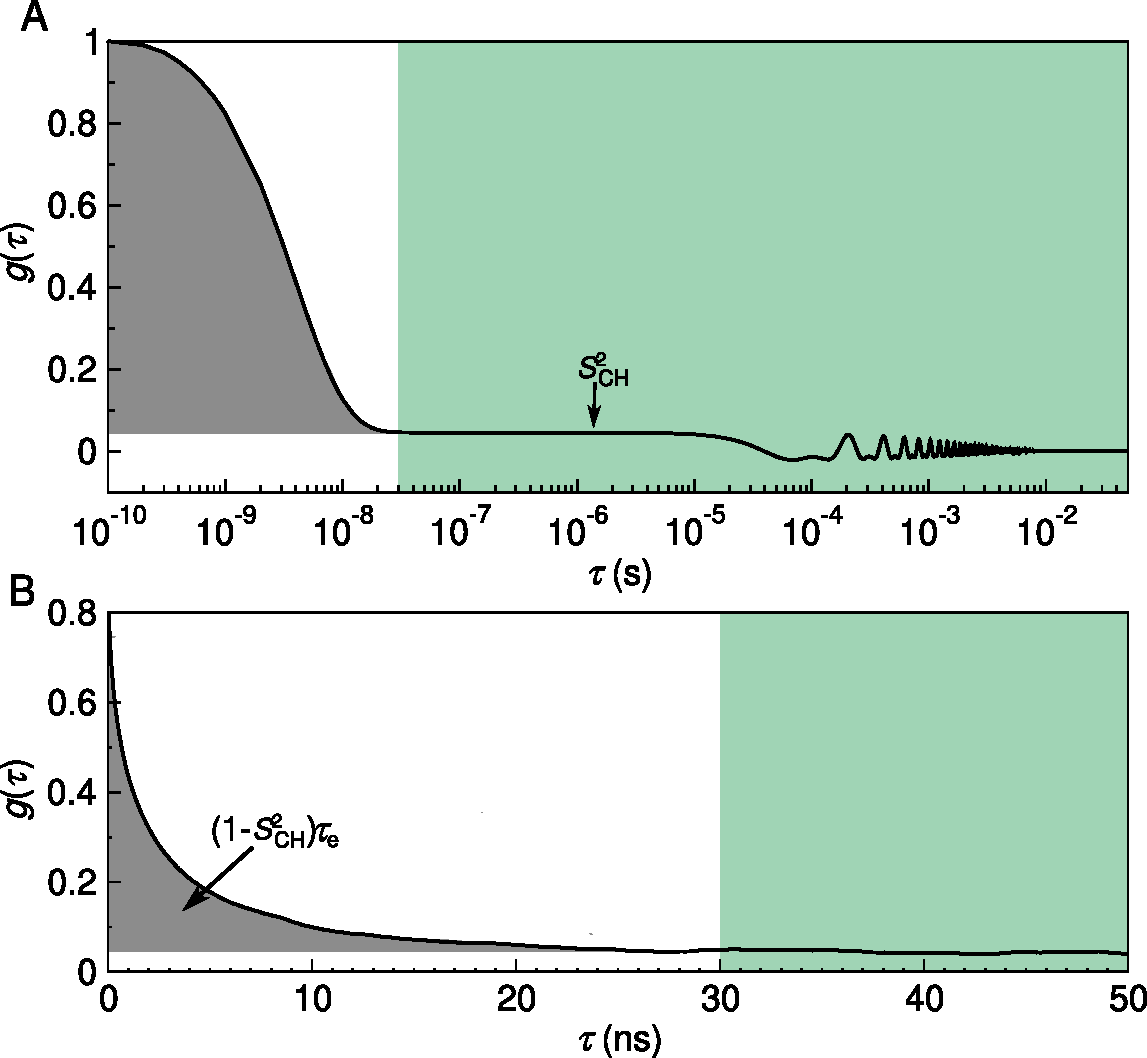
\includegraphics[scale=0.45]{../Figs/gfun_draft.pdf} 
\caption{C--H bond autocorrelation function $g(\tau)$. (A) Idealised illustration of the fast (white background) and the slow (green) mode of the correlation function. The fast mode decays to a plateau on which $g(\tau)=S^2_{\mathrm{CH}}$, while the slow mode gives the final descent to zero. Oscillations at the slow mode region are due to magic angle spinning. (B) Typical $g(\tau)$ obtained from an MD simulation, showing the decay towards $S^2_{\mathrm{CH}}$. The gray area under the curve is equal to $(1-S^2_{\mathrm{CH}})\tau_\mathrm{e}$. }
\label{fig:schem_teff}
\end{figure} 



\subsubsection*{Spin-lattice relaxation rates $R_1$.}
The \mbox{C--H} bond dynamics relate to $R_1$, the spin-lattice relaxation rate, through
\begin{align}
\label{eq:R1}
\begin{split}
R_{1}=&\frac{d^2_{\mathrm{CH}}N_{\mathrm{H}}}{20}\left[j(\omega_{\mathrm{H}}-\omega_{\mathrm{C}})\right. \\
&\left.+3j(\omega_{\mathrm{C}})+6j(\omega_{\mathrm{H}}+\omega_{\mathrm{C}})\right],
\end{split}
\end{align}
where $\omega_{\mathrm{H}}$ is the $^1$H and $\omega_{\mathrm{C}}$ the $^{13}$C-NMR Larmor frequency, and $N_{\mathrm{H}}$ the number of hydrogens covalently bonded to the carbon.
The rigid dipolar coupling constant $d_{\mathrm{CH}}\approx-2\pi\times22$\,kHz for the methylene bond.
%\todo{Why there is a minus sign above? TMF: because the horns of the Pake pattern come from the 90 degree orientation of the rigid C-H bond and P2(cos(90)) is negative. this is the convention in NMR simulation programs. not an important detail and skipping the negative sign is also fine.}
%$^{13}$C NMR experiments investigating lipid conformational dynamics take advantage of the fact that the relaxation of $^{13}$C magnetization dominantly happens via the dipolar coupling of the carbon with the magnetic moments of the protons bound to it, with the symmetry axis of the interaction aligning with the C--H bond.
The spectral density $j(\omega)$ is given by the Fourier transformation
%depicting the $^{13}$C relaxation rates (at frequency $\omega$) is expressed as
\begin{equation}
j{(\omega)}=2\int_{0}^{\infty}\cos(\omega\tau)g(\tau)\,\mathrm d\tau
\end{equation}
of the C--H bond autocorrelation function $g(\tau)$ (Eq.~\eqref{eq:BCF}).
Clearly
the connection between $R_1$ and molecular dynamics is not straightforward;
the magnitude of $R_1$ does, however, reflect the relative significance of processes
with timescales near the inverse of $\omega_{\mathrm{H}}$ and $\omega_{\mathrm{C}}$. These two frequencies depend on the field strength used in the NMR experiments: Typically
$R_1$ is most sensitive to motions with time scales $\sim$0.1--10\,ns.
%
(In our experimental data~\cite{ferreira15,pham15,Volke:1995a,Antila:2020a}
$\omega_\mathrm C=125$\,MHz and $\omega_\mathrm H=500$\,MHz,
which gives
$(2\pi\times125~\mathrm{MHz})^{-1}=1.3$\,ns and
$(2\pi\times625~\mathrm{MHz})^{-1}=0.25$\,ns.)
%
A change in $R_{1}$, therefore, indicates a change in the relative amount of processes
occurring in a window around the sensitive timescale, but does not give information on the direction (speedup/slowdown) to which the processes changed.
% It is impossible to directly connect an increase/decrease of $R_1$ rates to speedup/slowdown of specific motions.
% This is because $R_1$ values are only sensitive to processes whose timescales fall within a certain window.


\begin{comment}
 The dipolar coupling constant $d_{\mathrm{CH}}$ is defined as

\begin{equation}
d_{\mathrm{CH}}=\frac{\hslash\gamma_{\mathrm{H}}\gamma_{\mathrm{C}}\mu_{0}}{4\pi\langle r^{3}_{\mathrm{CH}} \rangle} ,
\end{equation}

where $\hslash$ is the reduced Planck constant, $\gamma_{\mathrm{C}}$ and $\gamma_{\mathrm{H}}$ are the gyromagnetic constants for $^{1}H$ and $^{13}C$, $\mu_{0}$ is the vacuum permeability, and $\langle r^{3}_{\mathrm{CH}}\rangle$ denotes the average cubic length of the C-H bond.
\end{comment}

\subsection*{Data acquisition and analysis.}
%
All the experimental quantities used in this work were collected from the literature sources~\cite{ferreira15,pham15,Volke:1995a,Antila:2020a} cited at the respective figures.   

%\subsection*{Simulational data acquisition and analysis.}
%
The simulation trajectories were collected from the general-purpose open-access repository Zenodo (\url{zenodo.org}), with the majority of the data originating from the NMR\-lipids Project~\cite{botan15,catte16} (\url{nmrlipids.blogspot.fi}). The trajectories were chosen by hand based on how well the simulation conditions matched the available experimental data (lipid type, temperature, cholesterol content, hydration), and how precisely one could extract the quantities of interest from the trajectory (length of simulation, system size).
%
Table~\ref{tab:standr} lists the chosen trajectories of pure POPC (1-palmit\-oyl-2-oleoyl-glycero-3-phosphocholine) bilayers at/near room temperature and at full hydration;
Table~\ref{tab:chol} lists the trajectories with cholesterol; and
Table~\ref{tab:hydr} those with varying hydration.
Full computational details for each simulation are available at the cited Zenodo entry.

\begin{table}[t!]
\caption{Analyzed open-access MD trajectories of pure POPC lipid bilayers at full hydration.
Note that the temperature varied across these openly available simulation data, but in no case was $T$ lower than in the experiment. Thus, as dynamics slows down when temperature drops, any overestimation of $\tau_\mathrm{e}$ by MD (as typically seen in Fig.~\ref{fig:teff_R1}) would get worse if the simulations were done at the experimental 298\,K.
}
\begin{minipage}[t]{\columnwidth}
\resizebox{\columnwidth}{!}{
\begin{tabular}{lrrrrc}
%\hline
force field  &
$N_{\rm l}$\footnote{Number of POPC molecules.} &
$N_{\rm w}$\footnote{Number of water molecules.}  &
$T$\footnote{Simulation temperature.}(K) &
$t_{{\rm anal}}$\footnote{Trajectory length used for analysis.}(ns) &
files\footnote{Reference for the openly available simulation files.} \tabularnewline
\hline 
%Berger-POPC-07~\cite{ollila07a}
%	& 128 & 7290 & 298 & 50  & {[}\!\!\citenum{bergerFILESpopc}{]} \tabularnewline[1.0ex]
Berger-POPC-07~\cite{ollila07a} %\cite{berger97,bachar04}
	& 256 & 10240 & 300 & 300  & {[}\!\!\citenum{bergerFILESpopcT300}{]} \tabularnewline[1.0ex]	
CHARMM36~\cite{klauda10}
	& 256 & 8704 & 300 & 300 & {[}\!\!\citenum{charmm36filesT300}{]} \tabularnewline
%CHARMM36~\cite{klauda10}
%	& 34 & 1020 & 300 & 140 & {[}\!\!\citenum{charmm36filesHA}{]}\tabularnewline[1.0ex]
%MacRog~\cite{kulig15} 
%	&  128  & 6400 & 310 & 200  & {[}\!\!\citenum{macrogCHOLfiles}{]}\tabularnewline[1.0ex]
MacRog~\cite{kulig15} 
	&  128  & 5120 & 300 & 500  & {[}\!\!\citenum{macrogfilesT300}{]}\tabularnewline[1.0ex]
Lipid14 \cite{dickson14}
	& 72 & 2234 & 303 & 50 & {[}\!\!\citenum{lipid14files}{]}\tabularnewline[1.0ex]
Slipids~\cite{jambeck12b}
	& 200 & 9000 & 310 & 500  & {[}\!\!\citenum{slipidsFILESpopcchol}{]}\tabularnewline[1.0ex]
ECC~\cite{melcr18}
	& 128 & 6400 & 300 & 300  & {[}\!\!\citenum{eccFILESpopc}{]}\tabularnewline
\end{tabular}
}
\end{minipage}
\label{tab:standr}
\end{table}

\begin{table}[]
\caption{Analyzed open-access MD trajectories of cholesterol-containing POPC bilayers at full hydration.}
\begin{minipage}[t]{\columnwidth}
\resizebox{\columnwidth}{!} {
\begin{tabular}{lrrrrrrc}
%\hline
force field POPC/cholesterol &
$c_{{\rm chol}}$\footnote{Bilayer cholesterol content (mol \%).}  &
$N_{\rm chol}$\footnote{Number of cholesterol molecules.}  &
$N_{\rm l}$\footnote{Number of POPC molecules.} &
$N_{\rm w}$\footnote{Number of water molecules.}  &
$T$\footnote{Simulation temperature.}(K) &
$t_{{\rm anal}}$\footnote{Trajectory length used for analysis.}(ns) &
files\footnote{Reference for the openly available simulation files.} 
\tabularnewline
\hline 
Berger-POPC-07~\cite{ollila07a}
	& 0\%	& 0	& 128	& 7290  & 298  & 50 & {[}\!\!\citenum{bergerFILESpopc}{]} \tabularnewline
/H\"{o}ltje-CHOL-13~\cite{holtje01,ferreira13} 
	& 50\%	& 64	& 64		& 10314  & 298  & 50  & {[}\!\!\citenum{bergerFILESpopc50chol}{]} \tabularnewline[1.0ex]
%CHARMM36~\cite{klauda10} 
%	& 0\%	& 0 	& 128 	& 5120  & 303  & 140  & {[}\!\!\citenum{charmm36files}{]} \tabularnewline
%/CHARMM36~\cite{lim12} 
% 	& 50\%	& 80	& 80		& 4496  & 303  & 200  & {[}\!\!\citenum{charmm36files50perCHOL}{]} \tabularnewline[1.0ex]
CHARMM36~\cite{klauda10} 
	& 0\%	& 0 	& 200 	& 9000  & 310  & 500  & {[}\!\!\citenum{T310charmm36files}{]} \tabularnewline
/CHARMM36~\cite{lim12} 
 	& 50\%	& 200	& 200		& 18000  & 310  & 500  & {[}\!\!\citenum{T310charmm36files50perCHOL}{]} \tabularnewline[1.0ex]
MacRog~\cite{kulig15}
	& 0\%	& 0	& 128	& 6400  & 310  & 500  & {[}\!\!\citenum{macrogCHOLfiles}{]} \tabularnewline
/MacRog~\cite{kulig15}
 	& 50\%	& 64	& 64		& 6400  & 310  & 500  & {[}\!\!\citenum{macrogCHOLfiles}{]} \tabularnewline[1.0ex]
Slipids~\cite{jambeck12b}
	& 0\%	& 0	& 200	& 9000 & 310 & 500  & {[}\!\!\citenum{slipidsFILESpopcchol}{]} \tabularnewline
/Slipids~\cite{jambeck13chol}
 	& 50\%	&200& 200	& 18000 & 310 & 500 & {[}\!\!\citenum{slipidsFILESpopcchol}{]}\tabularnewline
\end{tabular}
}
\end{minipage}
\label{tab:chol}
\end{table}

\begin{table}[]
\caption{Analyzed open-access MD trajectories of PC lipid bilayers under varying hydration level.}
\begin{minipage}[t]{\columnwidth}
\resizebox{\columnwidth}{!} {
\begin{tabular}{llrrrrrc}
%\hline
force field  &
lipid  &
$n_{{\mathrm w\!}_{/\mathrm l}}$\footnote{Water/lipid molar ratio.}  &
$N_{\rm l}$\footnote{Number of lipid molecules.}  &
$N_{\rm w}$\footnote{Number of water molecules.} &
$T$\footnote{Simulation temperature.}(K)  &
$t_{{\rm anal}}$\footnote{Trajectory length used for analysis.}(ns) &
files\footnote{Reference for the openly available simulation files.} \tabularnewline
\hline 
Berger-POPC-07~\cite{ollila07a} 
	& POPC  & 57  & 128  & 7290  & 298  & 50 & {[}\!\!\citenum{bergerFILESpopc}{]} \tabularnewline
	& POPC  & 7  & 128  & 896  & 298  & 60  & {[}\!\!\citenum{bergerDEHYDfiles}{]} \tabularnewline	
%Berger~\cite{berger97,bachar04}
	& POPC & 40 & 256 & 10240 & 300 & 300  & {[}\!\!\citenum{bergerFILESpopcT300}{]} \tabularnewline[1.0ex]		
Berger-DLPC-13~\cite{kanduc13}
	& DLPC\footnote{1,2-dilauroyl-sn-glycero-3-phosphocholine. \label{fn:DLPC}}  & 24  & 72  & 1728  & 300  & 80  & {[}\!\!\citenum{bergerFILESdlpc24}{]} \tabularnewline
	& DLPC\footref{fn:DLPC}  & 16  & 72  & 1152  & 300  & 80  & {[}\!\!\citenum{bergerFILESdlpc16}{]} \tabularnewline
	& DLPC\footref{fn:DLPC}  & 12  & 72  & 864  & 300  & 80  & {[}\!\!\citenum{bergerFILESdlpc12}{]} \tabularnewline
	& DLPC\footref{fn:DLPC}  & 4  & 72  & 288  & 300  & 80  & {[}\!\!\citenum{bergerFILESdlpc4}{]} \tabularnewline[1.0ex]
	
CHARMM36\cite{klauda10} 
	& POPC  & 40  & 128  & 5120  & 303  & 140 & {[}\!\!\citenum{charmm36files}{]} \tabularnewline
	& POPC  & 34	&  128  & 5120 & 300 & 500  & {[}\!\!\citenum{macrogfilesT300}{]}\tabularnewline[1.0ex]	
	& POPC  & 31 & 72 & 2232 & 303 & 20 & {[}\!\!\citenum{charmm36files31wPERl}{]}\tabularnewline[1.0ex]	
	& POPC  & 15  & 72  & 1080  & 303  & 20  & {[}\!\!\citenum{charmm36files15wPERl}{]} \tabularnewline
	& POPC  & 7  & 72  & 504  & 303  & 20  & {[}\!\!\citenum{charmm36files7wPERl}{]} \tabularnewline[1.0ex]
MacRog\cite{kulig15} 
	& POPC  & 50  & 288  & 14400  & 310  & 40  & {[}\!\!\citenum{macrogdehydFILES}{]} \tabularnewline
	& POPC  & 25  & 288  & 7200  & 310  & 50  & {[}\!\!\citenum{macrogdehydFILES}{]} \tabularnewline	
	& POPC  & 15  & 288  & 4320  & 310  & 50 & {[}\!\!\citenum{macrogdehydFILES}{]} \tabularnewline
	& POPC  & 10  & 288  & 2880  & 310  & 50  & {[}\!\!\citenum{macrogdehydFILES}{]} \tabularnewline
	& POPC  & 5  & 288  & 1440  & 310  & 50  & {[}\!\!\citenum{macrogdehydFILES}{]} \tabularnewline
\end{tabular}
}
\label{tab:hydr}
\end{minipage}

\end{table}
\begin{comment}
%\begin{multicols}{2}
%\twocolumn
\begin{table}[]
\caption{Analyzed simulations of POPC lipid bilayers at varying NaCl concentration.}
\begin{minipage}[t]{\columnwidth}
\resizebox{\columnwidth}{!} {
\begin{tabular}{lrrrrrrc}
%\hline
force field POPC/ions &
{[}NaCl{]}\footnote{NaCl concentration, calculated as
{[}NaCl{]}$=N_{{\rm Na}}\times${[}water{]}$/N_{{\rm w}}$, where {[}water{]} = 55.5\,M.} (mM)  &
$N_{{\rm Na}}$\footnote{Number of Na$^+$ ions, equal to number of Cl$^-$ ions.}   &
$N_{\rm l}$\footnote{Number of POPC molecules.}   &
$N_{\rm w}$\footnote{Number of water molecules.} &
$T$\footnote{Simulation temperature.}(K) &
$t_{{\rm anal}}$\footnote{Trajectory length used for analysis.}(ns) &
files\footnote{Reference for the openly available simulation files.}\tabularnewline
\hline 
CHARMM36\cite{klauda10}%/---
	&0	&0	&128	& 5120	&303	&140	& {[}\!\!\citenum{charmm36files}{]}\tabularnewline
%CHARMM36\cite{klauda10}
/CHARMM36\cite{venable13}
	&346	&13	& 72	& 2085	&303	& 60	& {[}\!\!\citenum{charmmPOPC350mMNaClfiles}{]} \tabularnewline
%CHARMM36\cite{klauda10}/CHARMM36\cite{venable13}
	&692	&26	& 72	& 2085	&303	& 60	& {[}\!\!\citenum{charmmPOPC690mMNaClfiles}{]} \tabularnewline
%CHARMM36\cite{klauda10}/CHARMM36\cite{venable13}
	&947	&37	& 72	& 2168	&303	& 60	& {[}\!\!\citenum{charmmPOPC950mMNaClfiles}{]} \tabularnewline[1.0ex]

MacRog\cite{kulig15}%/---
	&0	&0	&128	& 6400	&310	&500	& {[}\!\!\citenum{macrogCHOLfiles}{]}\tabularnewline
%MacRog\cite{kulig15}
/OPLS\cite{aqvist90}
	&103	&27	&288	& 14554	&310	& 50	& {[}\!\!\citenum{macrogIONfiles}{]} \tabularnewline
%MacRog\cite{kulig15}/OPLS\cite{aqvist90}
	&207	&54	&288	& 14500	&310	& 50	& {[}\!\!\citenum{macrogIONfiles}{]} \tabularnewline
%MacRog\cite{kulig15}/OPLS\cite{aqvist90}
	&311	&81	&288	& 14446	&310	& 40	& {[}\!\!\citenum{macrogIONfiles}{]} \tabularnewline
%MacRog\cite{kulig15}/OPLS\cite{aqvist90}
	&416	&108	&288	& 14392	&310	& 50	& {[}\!\!\citenum{macrogIONfiles}{]} \tabularnewline[1.0ex]

Slipids \cite{jambeck12b}%/---
	&0	&0	&200	& 9000	&310	&500	& {[}\!\!\citenum{slipidsFILESpopcchol}{]}\tabularnewline
%Slipids\cite{jambeck12b}
/AMBER\cite{smith94}
	&130	& 21	&200	& 9000	&310	&100	& {[}\!\!\citenum{slipidsFILESpopc130mMnaclSD}{]} \tabularnewline
%Slipids\cite{jambeck12b}/AMBER\cite{smith94}
	&999	&162	&200	& 9000	&310	&200	& {[}\!\!\citenum{slipidsFILESpopc1MnaclSD}{]}\tabularnewline
\end{tabular}
}
\end{minipage}
\label{tab:salt}
\end{table}
%\onecolumn
%\end{multicols}
\end{comment}

The trajectories were analyzed using in-house scripts. These are available on GitHub (\url{github.com/hsantila/Corrtimes/tree/master/teff_analysis}), along with a Python notebook outlining an example analysis run.  To enable automated analysis of several force fields with differing atom naming conventions, we used the mapping scheme developed within the NMR\-lipids Project to automatically recognise the atoms and bonds of interest for each  trajectory.

After downloading the necessary files from Zenodo, we processed the trajectory with Gromacs \texttt{gmx trjconv} to make the molecules whole.
We then calculated the  $S_\mathrm{CH}$ (Eq.~\eqref{eq:OP}) with the \texttt{OrderParameter.py} script that uses the MDanalysis\cite{agrawal11,gowers16} Python library.
%
The \mbox{C--H} bond correlation functions
$g(\tau)$ (Eq.~\eqref{eq:BCF})
were calculated with Gromacs\,5.1.4~\cite{abraham2015gromacs} \texttt{gmx rotacf}
(note that in MD $g_\mathrm s =1$ so that $g = g_\mathrm{f}$)
after which the $S_\mathrm{CH}$ were used to
normalize the $g_\mathrm f$ to obtain %the $g'_\mathrm f$, following Eq.~\eqref{eq:nBCF}.
the reduced and normalized correlation function
\begin{equation}
\label{eq:nBCF}
g'_{\mathrm{f}}(\tau)=\frac{g_{\mathrm{f}}(\tau)-S^{2}_{\rm{CH}}}{1-S^2_{\mathrm{CH}}},
\end{equation}
that is, the integrand in Eq.~\eqref{eq:teff}. 

The effective correlation times $\tau_\mathrm e$ were then calculated by integrating $g'_\mathrm f(\tau)$
from $\tau=0$ until $\tau = t_0$.
Here, $t_\mathrm 0$ is the first time point at which $g'_\mathrm f$ reached zero: $t_0 = \min
	\{
	t\,|\,g'_\mathrm f(t)=0
	\}
$.
%
If $g'_\mathrm f$ did not reach zero within 
$t_\mathrm{anal}/2$, the 
$\tau_\mathrm e$ was not determined,
and we report only its upper and lower estimates.

To quantify the error on $\tau_\mathrm e$, we first estimate the error on $g'_\mathrm f(\tau)$,
%At a given timepoint $\tau$,
where we account for two sources of uncertainty: $g_{\mathrm{f}}(\tau)$ and $S^2_\mathrm{CH}$.
%
Performing linear error propagation on Eq.~\eqref{eq:nBCF} gives
\begin{align}
\begin{split}
\label{eq:error}
\Delta g'_{\mathrm{f}}(\tau)
%=
%\frac{\mathrm d g'_\mathrm{f}(\tau)}{\mathrm d g_{\mathrm{f}}(\tau)}\Delta g_{\mathrm{f}}(\tau)
%+
%\frac{\mathrm d g'_\mathrm{f}(\tau)}{\mathrm dS_\mathrm{CH}}\Delta S_\mathrm{CH}
=
&\left|
	\frac{1}{1-S^2_\mathrm{CH}}
\right|
\Delta g_{\mathrm{f}}(\tau)\\
&+\\
&\left|
	\frac{2\left(g_\mathrm{f}(\tau)-1\right)S_\mathrm{CH}}{\left(1-S^2_\mathrm{CH}\right)^2}
\right|
\Delta S_\mathrm{CH}.
\end{split}
\end{align}
Here the $\Delta S_\mathrm{CH}$ was determined 
as the standard error of the mean of the $S_\mathrm{CH}$ over the $N_\mathrm l$ individual lipids in the system~\cite{botan15}.
%
Similarly, we quantified the error on $g_{\mathrm{f}}(\tau)$
by first determining the correlation function $g^m_{\mathrm{f}}(\tau)$ for each individual lipid $m$
over the whole trajectory, and then obtaining the error estimate
$\Delta g_{\mathrm{f}}(\tau)$
as the standard error of the mean over the $N_\mathrm l$ lipids.
%
Importantly, this gives an uncertainty estimate for $g_{\mathrm{f}}(\tau)$ at each time point $\tau$.

To obtain the lower bound on $\tau_\mathrm e$, we integrate the function
$g'_{\mathrm{f}}(\tau) - \Delta g'_{\mathrm{f}}(\tau)$ over time from $\tau=0$ until $\tau=t_\mathrm l$.
Here
\begin{equation}
t_\mathrm l= \min
\left\{
	\left\{
		t\,|\,g'_{\mathrm{f}}(t) - \Delta g'_{\mathrm{f}}(t) = 0
	\right\},
	\frac{t_\mathrm{anal}}{2}
\right\}.
\end{equation}
That is,
$t_\mathrm l$ equals
the first time point at which the lower error estimate of $g'_\mathrm f$ reached zero;
or $t_\mathrm l=t_\mathrm{anal}/2$, if zero was not reached before that point.
%This is the one sigma error.

To obtain the upper error estimate on $\tau_\mathrm e$, we first integrate the function
$g'_{\mathrm{f}}(\tau) + \Delta g'_{\mathrm{f}}(\tau)$ over time from $\tau=0$ until
$
t_\mathrm u= \min
\left\{
	t_0,
	{t_\mathrm{anal}}/{2}
\right\}.
$
Note, however,
that this is not yet sufficient, because there could be slow processes that our simulation was not
able to see. Although these would contribute to $\tau_\mathrm e$ with a low weight,
their contribution over long times could still add up to a sizable effect on $\tau_\mathrm e$.
%
That said, it is feasible to assume (see Fig. \ref{fig:schem_teff}A) that there are no longer-time contributions
to $g_\mathrm f$ than something that decays with a time constant of $10^{-6}$\,s.
%
We use this as our worst case estimate to assess the upper bound for $\tau_\mathrm e$, that is,
%
we assume that all the decay of $g_\mathrm f$ from the time point
$
t_\mathrm u$ %=\min
%\left\{
%	t_0,
%	{t_\mathrm{anal}}/{2}
%\right\}
%$
onwards comes solely from this hypothetical slowest process that decays with a time constant of $10^{-6}$\,s.
%
The additional contribution to the upper bound for $\tau_\mathrm e$ then reads
\begin{align}
\label{eq:extraUpperError}
\begin{split}
( g'_\mathrm f(t_\mathrm u)&+\Delta g'_\mathrm f(t_\mathrm u) )\\
&\times \underbrace{\int_{t_\mathrm u}^{10^{-6}\,\mathrm s} \exp\left(-\frac{\tau-t_\mathrm u}{10^{-6}\,\mathrm s}\right)\mathrm{d}\tau}_{= \left( 1 - \exp\left( \frac{t_\mathrm u-10^{-6}\,\mathrm s}{10^{-6}\,\mathrm s} \right) \right) 10^{-6}\,\mathrm s}.
\end{split}
\end{align}

%The effective correlation times $\tau_\mathrm e$ were calculated by integrating, see Eq.~\eqref{eq:teff}, $g'_\mathrm f(\tau)$ over time from $\tau=0$ until $\tau = t_0$.

The $R_{1}$ rates were calculated using Eq.~\eqref{eq:R1}.
%
The spectral density $j(\omega)$ was obtained from the normalized correlation function $g'_\mathrm f$
by fitting it with a sum of 61 exponentials
\begin{equation}
\label{eq:weights}
g'_\mathrm{f}(\tau)\approx\sum_{i=1}^{61}\alpha_{i}e^{-\tau/\tau_{i}},
\end{equation}
with logarithmically spaced time-scales $\tau_{i}$ ranging from 1\,ps to 1\,$\mu$s, 
and then calculating the spectral density of this fit
based on the Fourier transformation\cite{ferreira15}
\begin{equation}
\label{eq:j}
j{(\omega)}=2(1-S_\mathrm{CH})\sum_{i=1}^{61}\alpha_{i}\frac{\tau_{i}}{1+\omega\tau_{i}} .
\end{equation}
%
The $R_{1}$ rate of a given C--H pair was
first calculated separately for each lipid $m$ (using Eq.~\eqref{eq:R1} with $N_\mathrm{H}=1$, and $j^m(\omega)$ obtained for the normalized correlation function ${g'_\mathrm f}^m$). The resulting $N_\mathrm{l}$ measurements per \mbox{C--H} pair were then assumed independent:
Their mean gave the $R_1$ rate of the C--H pair, and 
standard error of the mean its uncertainty.
%
The total $R_1$ rate of a given carbon was obtained as a sum of the $R_1$ rates of its C--H pairs.
%
When several carbons contribute to a single experimental $R_1$ rate due to the overlapping peaks (for example in C2 carbon in the acyl chains and the $\gamma$ carbons),
the $R_1$ from simulations was obtained as an average over carbons with overlapping peaks.
%
The segment-wise error estimates were obtained by standard error propagation, starting from the uncertainties of the $R_1$ rates of the C--H pairs.

To gain some qualitative insight on the time scales at which the main contributions to the $R_{1}$ rates arise,
we also calculated 'cumulative' $R_1$ rates, $R_1(\tau)$, which contained those terms of the sum in Eq.~\eqref{eq:j} for which $\tau_i<\tau$.
Note that here the $g'_\mathrm{f}$ averaged over lipids was used;
therefore, the 'cumulative' $R_1(\tau\to\infty)$ does not necessarily have exactly
the same numerical value as the actual $R_1$.

Finally, we note that the fit of Eq.~\eqref{eq:weights} provides an alternative
to estimating $\tau_\mathrm{e}$, because
\begin{equation}
\label{eq:TeffSum}
\tau_\mathrm{e}
	=\int_0^\infty\!g'_\mathrm f(\tau)\,\mathrm d\tau
	\approx\sum_{i}\alpha_{i}\tau_{i}.
\end{equation}
When the simulation trajectory is not long enough for the correlation function to reach the plateau, integrating $g'_\mathrm f$ gives a lower bound estimate for $\tau_\mathrm{e}$, while the sum of Eq.~\eqref{eq:TeffSum} includes also (some) contribution from the longer-time components via the fitting process.
However, in practice the fit is often highly unreliable in depicting the long tails of the correlation function, and thus we chose to quantify $\tau_\mathrm{e}$ using the area under $g'_\mathrm f$, and estimate its uncertainty as detailed above.

\section{Results and Discussion}
\begin{comment}
The internal dynamics of lipids in MD simulations has been previously evaluated by comparing
the $^2$H or $^{13}$C spin relaxation times, or effective correlation times calculated from simulation
trajectory with the experimental data \cite{feller02,wohlert06,klauda08,klauda08II,ferreira15,Ollila:2016a}.
As lipids exhibit complex internal dynamics with multiple timescales that cannot be fully captured
with a single parameter, several experimental quantities, detected for example with different
magnetic fields or temperatures, are required to fully evaluate dynamics in simulations or to interpret dynamics
from experiments \cite{Roberts:2009a,leftin11}.
\end{comment}

Using open-access MD simulation trajectories,
we benchmark phospholipid conformational  dynamics in six
MD force fields. %Berger, Slipids, MacRog, Lipid14, ECC, and CHARMM36
We start with
pure POPC bilayers in their liquid crystalline fully hydrated state
(see Table~\ref{tab:standr} for simulation details and Fig.~\ref{fig:teff_R1} for the data), and
% We
then proceed to
%cover a wider range of experimentally, biologically, and computationally relevant conditions, where we explore
check the changes in dynamics when cholesterol is added to the bilayer (Table~\ref{tab:chol} and Fig.~\ref{fig:chol}) and when the hydration level is reduced (Table~\ref{tab:hydr} and Fig.~\ref{fig:hydration}).
%We compared against
Our yardsticks are
the effective correlations times $\tau_\mathrm e$ (Eq.~\eqref{eq:teff}) and
the $R_1$ rates (Eq.~\eqref{eq:R1})
measured at 125\,MHz $^{13}$C (500\,MHz $^1$H) Larmor frequency;
an MD model with correct rotational dynamics in a window around $\sim$1\,ns
%$(2\pi\times125~\mathrm{MHz})^{-1}=1.3$\,ns and
%$(2\pi\times625~\mathrm{MHz})^{-1}=0.25$\,ns
will match the experimental $R_1$ rates, whereas
the $\tau_\mathrm{e}$ reflect all the sub-$\mu$s time scales (Fig.~\ref{fig:schem_teff}).



%\subsection*{Effective correlation times $\tau_\mathrm e$ at standard conditions.}
\subsection*{Pure POPC at full hydration: Slipids and CHARMM36 reproduce $\tau_\mathrm e$ excellently.}
The top panels of Fig.~\ref{fig:teff_R1} compare the effective correlation times $\tau_\mathrm{e}$ obtained for fully hydrated POPC bilayers in experiments (black) and in six different MD force fields (color).
We see that---as implied by the discussion leading to Eq.~\eqref{eq:extraUpperError}---sub-$\mu$s MD simulations typically lead to asymmetric error bars on $\tau_\mathrm{e}$;
if these open-access trajectories were extended,
the $\tau_\mathrm{e}$ values would more likely increase than decrease.
Qualitatively, every force field captures the general shape of the $\tau_\mathrm{e}$ profile: Dynamics slows down towards the glycerol backbone in both the headgroup and the tails.

Quantitatively, most MD simulations tend to produce too slow dynamics in the glycerol region (Fig.~\ref{fig:teff_R1}).
This %detected slow glycerol backbone dynamics in MD
is consistent with previous results for the Berger model~\cite{ferreira15}, and with the
insufficient conformational sampling of glycerol backbone torsions observed in 500-ns-long CHARMM\-c32b2~\cite{schlenkrich96,feller00} simulations of a PC lipid~\cite{vogel12}. %DOPC

The best overall $\tau_\mathrm{e}$-performance is seen in
Slipids and in particular CHARMM36 (Fig.~\ref{fig:teff_R1}). %---although the $\tau_\mathrm{e}$ in Slipids exhibit a qualitatively wrong (decreasing) trend from $\mathrm g_{3}$ to $\mathrm g_{1}$.
%
This is in line with CHARMM36 reproducing the most realistic conformational ensembles
for the headgroup and glycerol backbone among the MD simulation force fields benchmarked here~\cite{botan15,Antila:2019a}.
%
Indeed, it is important to keep in mind that the conformational ensembles %of glycerol backbone and headgroup 
greatly differ between  force fields and are not exactly correct in any of them~\cite{botan15,Antila:2019a}.
Consequently, the calculated $\tau_\mathrm{e}$ times and $R_1$ rates
depict the dynamics of sampling a somewhat different and incorrect phase space
for each model. %that differs from what is being observed in the experiments.
To this end, we try to avoid overly detailed discussion on the models and rather concentrate on common and qualitative trends.
That said,
there are a few carbon segments in the data for which
the experimental order parameters, $R_1$, and $\tau_\mathrm{e}$ are all (almost) reproduced by simulations,
suggesting that the conformational ensemble and dynamics is correctly captured by MD in these cases. 
For example, 
% LET'S MENTION ONLY THE VERY GOOD ONES,
% AND WHERE ALSO THE S_CH MATCH (although they are not shown)
% Lipid14, ECC, and MacRog perform well at the oleoyl double bond; % the S_CH are not within errors
Slipids performs well at the $\beta$ and $\alpha$, and
CHARMM36 at the g$_3$, g$_2$,  and C2 segments. % and % The C3 S_CH are not within exp error
These are, however, exceptions.

\begin{figure*}[!h]
\centering
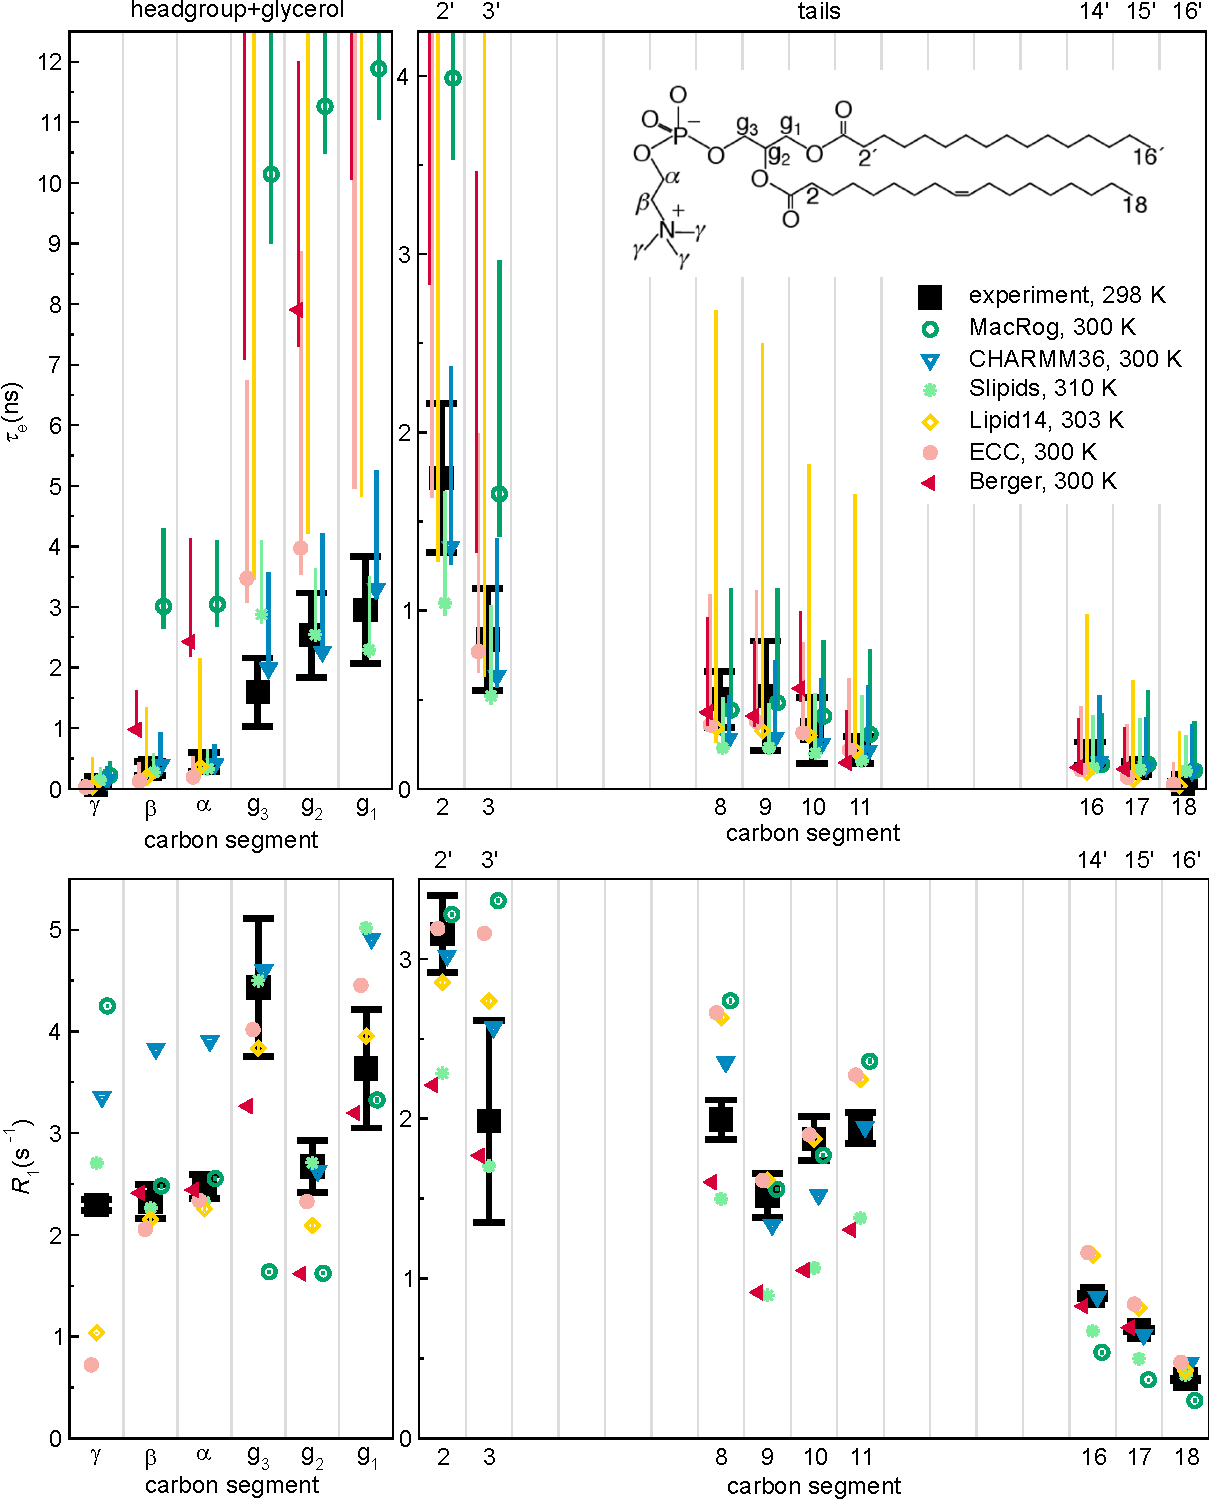
\includegraphics[width=0.81\textwidth]{../Figs/normalcond5.pdf}
\caption{Effective correlation times ($\tau_\mathrm{e}$, top) and $R_{1}$ rates (bottom) in experiments~\cite{Antila:2020a} (black) and MD simulations (colored) of POPC bilayers in $L_{\alpha}$ phase under full hydration.
Inset shows the POPC chemical structure and carbon segment labeling.
Each plotted value contains contributions from all the hydrogens within its carbon segment; the data for segments 8--11 are only from the sn-2 (oleoyl) chain, whereas the (experimentally non-resolved) contributions of both tails are included for segments 2--3 (2'--3' in the sn-1 chain) and 16--18 (14'--16').
%
Simulation results are only shown for the segments for which experimental data was available.
%
For $\tau_\mathrm{e}$,
a simulation data point indicates the average over C--H bonds; however,
if $\tau_\mathrm{e}$ could not be determined for all bonds, only the error bar
(extending from the mean of the lower to the mean of the upper error estimates) is shown.
%
The Berger data for segments $\gamma$, C18, and C16' are left out, as the protonation algorithm used to construct the hydrogens post-simulation in united atom models does not preserve the methyl C--H bond dynamics.
%
Table~\ref{tab:standr} provides further simulation details, while information on the experiments is available at Ref.~\citenum{Antila:2020a}.
}
\label{fig:teff_R1}

\end{figure*}

%\subsection*{$R_1$ rates at standard conditions.}
\subsection*{An excellent $\tau_\mathrm e$ may be accompanied by a poor $R_1$, or \emph{vice versa}.}
The lower panels of Fig.~\ref{fig:teff_R1} compare the experimental and simulated $R_{1}$ rates under the same conditions that were used for the $\tau_\mathrm{e}$ above.
%
\begin{comment}
There are certain qualitative features that all force fields predict correctly
(for example that $\mathrm g_2$ has the smallest $R_1$ among the glycerol and C9 among the oleoyl double bond segments),
and certain that they all miss (that $R_1$ rates for the oleoyl segments C8, C10, and C11 are all roughly equal).
\end{comment}
%
Notably, there are several instances where the $R_1$ comparison distinctly differs from what was seen for $\tau_\mathrm{e}$.

There are cases where
a matching $R_{1}$ is accompanied by a larger-than-experimental $\tau_\mathrm{e}$.
%Also examples to the contrary are seen: MacRog reproduces $R_{1}$ rates well for the $\beta$, $\alpha$, g$_3$, and g$_1$ segments, although it systematically overestimates their $\tau_\mathrm{e}$.
MacRog for the $\beta$, $\alpha$, and g$_1$ segments provides a prominent example
%where the $R_1$ rates are well reproduced, but $\tau_\mathrm e$ times systematically overestimated.
of this.
Such a combination suggests that MD has the correct relative weight of 1-ns-scale dynamics, but has too slow long-time dynamics.

There are also cases
%Some models that do very well for $\tau_\mathrm{e}$, do rather poorly for $R_1$. % such as CHARMM36 in the $\gamma$, $\beta$, and $\alpha$ segments. The opposite---
where $\tau_\mathrm{e}$ matches experiments, but $R_1$ does not, such as
the $\beta$ and $\alpha$ segments in CHARMM36.
Therein a cancellation of errors occurs in $\tau_\mathrm{e}$: The
overestimation of the relative weight of
1-ns-scale dynamics is compensated by wrong dynamics at the other time scales.
As CHARMM36 overall performs rather well for C--H bond order parameters, $R_1$, and $\tau_\mathrm{e}$,
we proceed to study this shortcoming on the headgroup $R_1$ rates
in some more detail.
%
%Berger and Slipids for tail segment 2.

%In the tail region, the MD models are in somewhat worse agreement with $R_{1}$ rates than what was seen for $\tau_\mathrm{e}$.
%General tendency for MD to succeed in shorter time scales whereas rotations with slower dynamics are not depicted as well?

%\subsection*{Dynamics of headgroup segments in CHARMM36.}
\subsection*{Conformational dynamics of PC headgroup segments in MD.}

Figure~\ref{fig:cumulativeR1s}A zooms in on the headgroup ($\gamma$, $\beta$, $\alpha$) segments,
whose $\tau_\mathrm e$ were not clearly visible on the scale of Fig.~\ref{fig:teff_R1}.
%
We see that for $\gamma$,
no force field provides both $\tau_\mathrm e$ and $R_1$,
but Slipids comes closest.
%
For $\beta$ and $\alpha$,
%CHARMM36 matches the experimental $\tau_\mathrm e$, but overestimates $R_1$, while
Slipids captures both measurables near perfectly.  
%
In other words, among the benchmarked force fields Slipids gives the most realistic description of the conformational dynamics in the headgroup region.
CHARMM36, e.g., overestimates ($R_1$) the relative weight of timescales around $\sim$1\,ns.

\begin{figure}[!h]
\centering
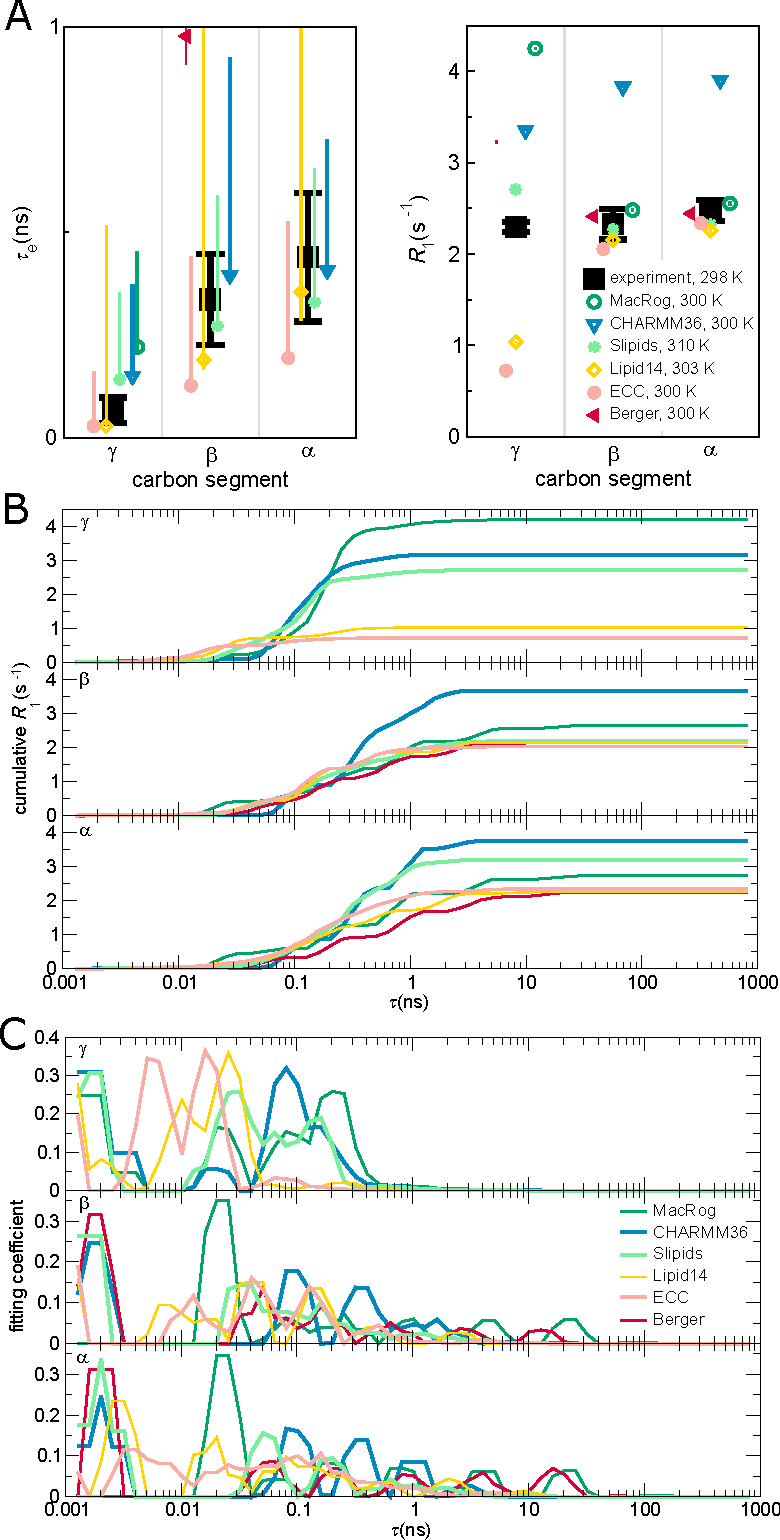
\includegraphics[width=\columnwidth]{../Figs/cumulativeR1.pdf}
\caption{Contributions to the dynamics of the headgroup segments.
(A) Zoom on the headgroup $\tau_\mathrm e$ (left panel) and $R_1$ (right).
(B) 'Cumulative' $R_1(\tau)$ of the
$\gamma$ (top panel), $\beta$ (middle), and $\alpha$ (bottom) segments.
$R_1(\tau)$ is obtained, as detailed in Methods,
by including in the sum of Eq.~\eqref{eq:j} only terms with $\tau_i<\tau$.
Consequently, at $\tau\to\infty$ the $R_1(\tau)$ approaches the actual $R_1$.
(C) Prefactor weighs $\alpha_i$ from Eq.~\eqref{eq:weights} of $\gamma$ (top), $\beta$ (middle), and $\alpha$ (bottom).
Note that panels B and C show a sliding average over 3 neighboring data points.
}
\label{fig:cumulativeR1s}
\end{figure}

To investigate closer how the differences between force fields arise, Fig.~\ref{fig:cumulativeR1s}B shows the 
'cumulative' $R_1(\tau)$, where the ranges of steepest increase indicate time scales that most strongly contribute to $R_1$ rates.

For the $\gamma$ segment,
Fig.~\ref{fig:cumulativeR1s}B shows
that for models that overestimate the $R_1$ rate 
(MacRog, CHARMM36, and Slipids, see Fig.~\ref{fig:cumulativeR1s}A)
the major contribution to $R_1$ arises at $\tau>50$\,ps, whereas for models that underestimate $R_1$ 
(Lipid14 and ECC)
the major contribution comes from $\tau<50$\,ps. 
%
This also manifests in the
distribution of fitting weights ($\alpha_i$ in Eq.~\eqref{eq:weights}) in Fig.~\ref{fig:cumulativeR1s}C:
The later non-zero weights occur, the larger is the resulting $R_1$ of $\gamma$.

For the $\beta$ and $\alpha$ segments, Fig.~\ref{fig:cumulativeR1s}B shows
that the main contribution to $R_1$ rates arises from processes
between 100\,ps and 1\,ns.
%
CHARMM36 has the largest relative weights of all models in this window (Fig.~\ref{fig:cumulativeR1s}C),
which explains its overestimation of $R_1$ of $\beta$ and $\alpha$.
%
All the other models have $R_1$ rates close to experiments,
but only Slipids simultaneously gives also the $\tau_\mathrm e$ correctly.
Notably, Slipids has its largest weights at $\tau<100$\,ps.
%
Indeed, the considerable weights
at short ($<10$\,ps) time scales  in all models except MacRog and
at long ($>10$\,ns) time scales in %both $\beta$ and $\alpha$ for
MacRog and Berger hardly manifest in $R_1$.
%
However, the latter contribute heavily to $\tau_\mathrm e$,
which is thus considerably overestimated by MacRog and Berger (Fig.~\ref{fig:teff_R1}).

It would be highly interesting to identify the origins of the observed artificial timescales,
particularly for the 0.1--1\,ns window over-presented in CHARMM36, and
propose how to correct those in the simulation models.
However, the connection between the fitted correlation times and the correlation times of distinct motional processes, such as dihedral rotations and lipid wobbling, turns out to be highly non-trivial; we thus refrain from further analysis here.

\subsection*{Effect of cholesterol.}
An essential component in cell membranes, cholesterol has various biological functions.
It is well known to order the acyl chains in lipid bilayers, but
its effect on the headgroup is more controversial~\cite{huang99,ferreira13}.
For example, it has been proposed that lipid headgroups
reorganize to shield cholesterol from water~\cite{huang99}. However, while acyl chains do substantially order,
NMR experiments show no significant conformational changes in the headgroup upon addition
of even 50\% of cholesterol---which
suggests that the tail and head regions behave essentially independently~\cite{ferreira13,botan15}.
In principle, the headgroups could shield cholesterol from water even
without changing their conformational ensemble: By reorienting only laterally on
top of the cholesterol. In this case, one would expect the rotational dynamics of headgroup segments to change when cholesterol is added.

Top panels of Fig.~\ref{fig:chol}A depict the experimental effective correlation times $\tau_\mathrm e$ in pure POPC bilayers and in bilayers containing 50\% cholesterol. The $\tau_\mathrm e$ at the glycerol backbone
slow down markedly when cholesterol is added. Tail segment dynamics slows down too, most notably close to the glycerol backbone.
%
In stark contrast,
$\tau_\mathrm e$ of the headgroup segments ($\gamma$, $\beta$, $\alpha$)
remain unaffected.
%
Furthermore, cholesterol induces no measurable change in the
headgroup $\beta$ and $\alpha$ segment
dynamics at short ($\sim$1\,ns) time scales, as
demonstrated by
the experimental $R_{1}$ rates (Fig.~\ref{fig:chol}A, bottom panels).
That said,
there is a small but measurable impact on $R_1$ at $\gamma$.
%
In summary, these experimental findings
%suggest that acyl chain ordering upon cholesterol addition is accompanied with slower internal dynamics in the hydrophobic core and the glycerol backbone regions, while the headgroup dynamics remains almost intact even with 50\% of cholesterol,
support the idea~\cite{Antila:2020a} that the acyl chains and the headgroup can respond
almost independently to changes in conditions and composition.

All four benchmarked force fields (Fig.~\ref{fig:chol}B) qualitatively reproduce the experimental increase in $\tau_\mathrm e$:
Slipids and CHARMM36 give rather decent magnitude estimates, while MacRog grossly overestimates the slowdown of glycerol, C2, and C3 segments. Notably, MacRog appears to predict slowdown also for the headgroup ($\beta$ and $\alpha$), for which experiments detect no change.
%
Note that  while CHARMM36 correctly shows no change in $\tau_\mathrm{e}$
of the $\gamma$, $\beta$, and $\alpha$ segments,
it does predict an erroneous $\Delta R_{1}$ for all three, indicating some inaccuracies in the
headgroup rotational dynamics. % at shorter time-scales.
Such inaccuracies might be reflected in the recent findings~\cite{leeb18}
(obtained using CHARMM36)
that 
%(at least at small cholesterol concentrations)
the headgroups of PCs neighboring (within 6.6\,\AA) a lone cholesterol  spend more time on top of the said cholesterol than elsewhere.
%\todo{Samuli wants to remove this, why? such arrested rotations could manifest on $\tau_\mathrm e$ and $R_1$.}
%
Interestingly, 
the tail $\Delta R_{1}$ seem to be qualitatively reproduced by
all three all-atom force fields, whereas Berger fails to capture the trend at the oleoyl double bond.
%
%Along with the slow-down of dynamics, all the models show an increase in the $\vert S_{\rm{CH}}\vert$ upon addition of cholesterol at the tail region (\todo{Show data?}), reflecting the reduced available volume for the POPC.\todo{Is this a known effect/explanation?}
%The change observed here, however, is particularly sensitive to the length of the trajectory as cholesterol-induced increase in effective correlation time is likely to lead to worse convergence of the correlation function within the limited simulation time, and more drastic underestimation of $\tau_\mathrm{e}$ is expected than for simulations without cholesterol. This will, consequently, cause a tendency towards underestimation on the strength of the cholesterol-driven modulation of the effective correlation time.
%
All these findings are
in line with the general picture obtained from C--H bond order parameters~\cite{Ollila:2016a}: MD simulations capture the changes
in acyl chain region rather well, but changes in and near the glycerol backbone region can be overestimated.
%
Of the benchmarked force fields, CHARMM36 appears most realistic in reproducing the effects of cholesterol on the glycerol backbone---and Slipids on the PC headgroup---conformational dynamics.

\begin{figure}[h!]
	\centering
	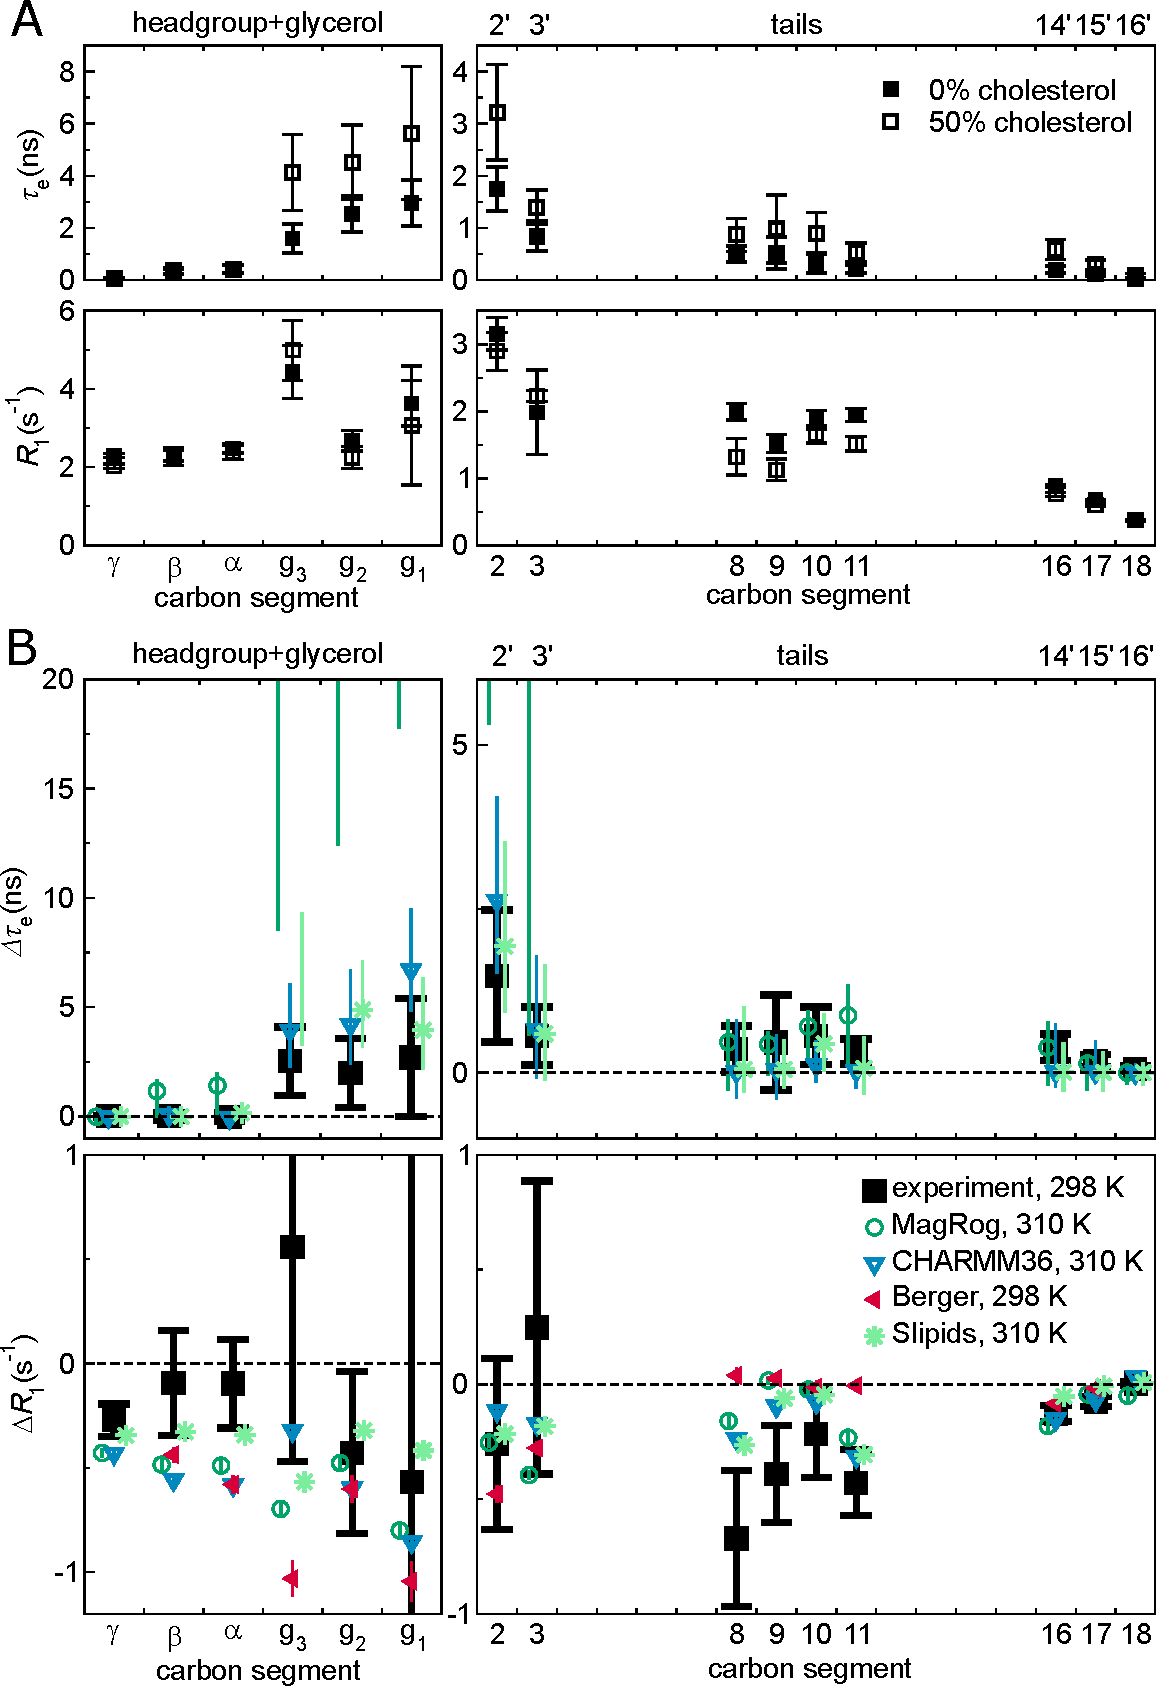
\includegraphics[width=\columnwidth]{../Figs/cholesterol.pdf}  
	\caption{Effect of cholesterol on POPC conformational dynamics.
	(A) Experimental effective correlation times $\tau_\mathrm{e}$ (top panels) and $R_{1}$ rates (bottom) in 100/0 and 50/50 POPC/cholesterol bilayers at full hydration, see Ref.~\citenum{Antila:2020a} for further details.
	(B) The change in $\tau_\mathrm{e}$ ($\Delta\tau_\mathrm{e}$, top panels) and $R_{1}$ ($\Delta R_{1}$, bottom),
	in NMR (black) and MD (color), when bilayer composition changes from pure POPC to 50\% cholesterol.
	Error estimates for the simulated $\Delta\tau_\mathrm e$ are the maximal possible
	based on the errors at 0\% and 50\% cholesterol;
	for other data regular error propagation is used.
	The Berger $\Delta\tau_\mathrm{e}$ is not shown, because the available open-access trajectories were too short to determine meaningful error estimates.
	Table~\ref{tab:chol} provides further simulation details;
	for segment labeling, see Fig.~\ref{fig:teff_R1}.
	}
	\label{fig:chol}
\end{figure}

\subsection*{Effect of drying.}
Understanding the impact of dehydration on the structure and dynamics of lipid bilayers is of considerable biological interest.
Dehydrated states are found, e.g., in skin tissue.
Most prominently, the process of membrane fusion is always preceeded by removal of water between the approaching surfaces, and thus the dehydration-imposed changes can considerably affect fusion characteristics, such as its rate.

Figure~\ref{fig:hydration}A shows how a mild dehydration affects
C--H bond dynamics in the PC headgroup and glycerol backbone;
the plot compares the experimental effective correlation times $\tau_\mathrm e$
measured for POPC at full hydration and for DMPC (1,2-dimyristoyl-sn-glycero-3-phosphocholine)
at 13 waters per lipid.
%
The $\tau_\mathrm e$ are the same within experimental accuracy, which suggests two conclusions. Firstly, 
the headgroup ($\gamma$, $\beta$, $\alpha$) $\tau_\mathrm e$ are rather insensitive to the chemical identities of the tails. This is analogous to  what was seen experimentally when adding cholesterol
(Fig.~\ref{fig:chol}A): Structural changes in the tail and glycerol regions do not (need to) affect the headgroup dynamics. Secondly, a mild dehydration does not alter the $\tau_\mathrm e$
in the headgroup and glycerol regions. 


\begin{figure*}[ht!]
\centering
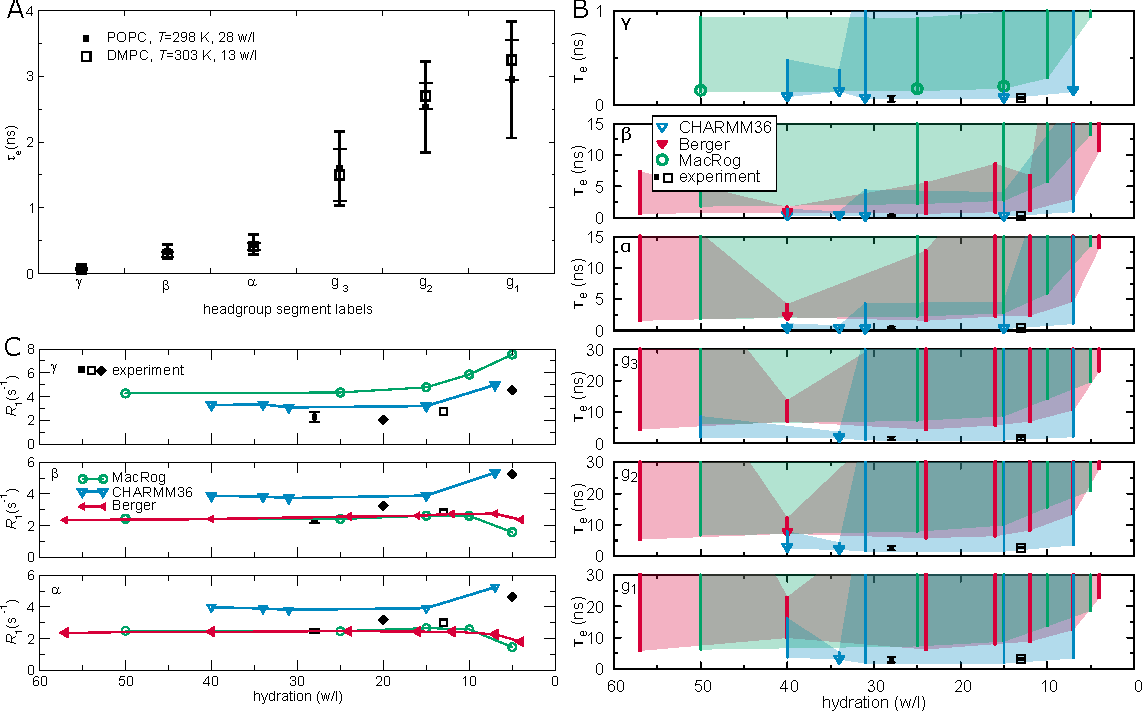
\includegraphics[width=\textwidth]{../Figs/hydration_2columns.pdf} 

\caption{Effect of drying on PC headgroup and glyc\-er\-ol backbone conformational dynamics.
(A) Experimental effective correlation times $\tau_\mathrm e$ for
DMPC at low hydration %(13\,w/l)
(from Ref.~\citenum{pham15})
do not significantly differ from the
$\tau_\mathrm e$ for POPC at full hydration (from Ref.~\citenum{Antila:2020a}). %(28\,w/l)
(B) Calculated $\tau_\mathrm e$  for
POPC at decreasing hydration in three MD models.
Symbols indicate the mean of segment hydrogens
if $\tau_\mathrm{e}$ could be determined for all of them; otherwise, only the error bar
(extending from the mean of the lower to the mean of the upper uncertainty estimates) is drawn.
The area limited by the error bars shaded for visualization.
Note that four Berger data points (4, 12, 16, and 24\,w/l) are from DLPC.
(C) $^{13}$C-NMR $R_1$ rates (at $\omega_\mathrm C=125$\,MHz) of the PC headgroup segments
in experiments and simulations: Experiments indicate an increasing trend upon dehydration. Experimental POPC data at 28 w/l is from Ref.~\citenum{Antila:2020a} ($\blacksquare$), POPC at 20 and 5\,w/l from Ref.~\citenum{Volke:1995a} ($\blacklozenge$), and DMPC at 13 w/l from Ref.~\citenum{pham15} ($\square$). 
See Table~\ref{tab:hydr} for simulation details.}
\label{fig:hydration}
\end{figure*}

Figure~\ref{fig:hydration}B shows the effects of dehydration in three MD models.
Combination of
the unrealistically slow dynamics, especially in the glycerol backbone (Fig.~\ref{fig:teff_R1}), and
the relatively short lengths of the available open-access trajectories %with dehydration conditions
(Table~\ref{tab:hydr})
led to large uncertainty estimates; %for simulation data are large. %which makes discussion challenging.
%owing to which,
thus we only point out qualitative trends here. For all headgroup and glycerol segments, the simulated  $\tau_\mathrm e$ indicate slowdown upon dehydration. This is manifested in the increase in the magnitude of the error estimate (cf. the Berger data for $\beta$ and $\alpha$) as well as in the increase of the lower limit of the error. 
For CHARMM36 the lower error estimates stay almost constant all the way until 7\,w/l, whereas for Berger and MacRog they hint that a retardation of dynamics starts already between 15 and 10\,w/l.

These simulational findings suggest that
experiments reducing hydration levels below 10\,w/l would also show an increase in $\tau_\mathrm e$.
This prediction is in line with the
exponential slow-down
%(decay constant $\sim$4 removed waters per lipid)
of the headgroup conformational dynamics
upon dehydration that was indicated by $^2$H-NMR $R_{1}$ measurements
of DOPC bilayers:
$R_1\sim\exp(-n_{{\mathrm w\!}_{\!/\mathrm l}}/4)$~\cite{ulrich94}.
%
The slowdown was attributed to the reduced effective volume available for the headgroup~\cite{ulrich94}
as it tilts towards the membrane upon dehydration;
such tilt is observed via changes of the lipid headgroup order parameters~\cite{bechinger91},
and is qualitatively reproduced by all the simulation models~\cite{botan15}.

%{\color{red} Cite also the D$_2$O data. \cite{Volke:1994b}}
%{\color{blue} There are also data for the tails. \cite{Volke:1982a}}
%{\color{green} Ref.~\citenum{Faure:1997a}: Each DMPC in fluid phase binds $\sim$10 D$_2$O.}


Figure~\ref{fig:hydration}C shows
a collection of experimental $^{13}$C-NMR $R_1$ rates
%measured at $\omega_\mathrm C=125$\,MHz
for the headgroup segments at different water contents;
in addition to the full hydration POPC data from Fig.~\ref{fig:teff_R1},
DMPC at 13\,w/l~\cite{pham15}, % 125 MHz, 300K
and POPC at 20 and 5\,w/l~\cite{Volke:1995a} %125.76 MHz, 298K
are shown.
%
Experimentally, an increasing trend with decreasing hydration is observed for all three segments,
indicating changes of headgroup dynamics at short ($\sim$1\,ns) time scales.
Interestingly, only CHARMM36 captures this,
whereas Berger and MacRog give decreasing $R_1$ rates for $\beta$ and $\alpha$.
%

The slowdown characteristics discussed here are of significance
not only for computational studies of inter\-membrane interactions, such as fusion,  but also when simulating a bilayer (stack) under low hydration: Slower dynamics require longer simulation times for equilibration, for reliably quantifying the properties of the bilayers, and for observing rare events. %such as the lipid tail flips from one membrane to another in case of the fusion~\cite{best citation here}. Same applies in simulations performed in increasing concentrations of cholesterol, as the slow down of dynamics and the increase of tail order parameters observed therein are analogous to those occurring upon dehydration. \todo{really not the smoothest text}
%Sims by Calero~\cite{Calero:2019a} for water dynamics at membrane

\section{Conclusions}
%ONNISTUU.
%LYHYITA SIMUJA VOISI JATKAA, MUTTA TASSA SITA EI TEHTY DEMOAMISEN TAKIA.
Open access databanks of MD trajectories enables the creation new scientific information without running a single new simulation. Here,
we demonstrated this by investigating the dynamics of a wide range of phosphatidylcholine molecular dynamics models using the existing trajectories from the NMRlipids databank.

We found that MD qualitatively captures the $^{13}$C-NMR effective correlation time ($\tau_\mathrm e$) profile of POPC---the slow glycerol backbone and the faster motions of the headgroup and tail regions---but most MD force fields are prone to too slow dynamics of the glycerol C--H bonds (Fig.~\ref{fig:teff_R1}).
%
While no force field perfectly reproduces all the experimental data,
CHARMM36 and Slipids have an overall impressive $\tau_\mathrm e$.
This is particularly true for CHARMM36, as it is also known to
well represent the experimental conformational ensemble~\cite{botan15}.
%
That said, we find that CHARMM36 struggles with the balance of dynamics in the headgroup region:
The $R_1$ rates, sensitive for $\sim$1-ns processes, are too high for the $\gamma$, $\beta$, and $\alpha$ segments (Fig.~\ref{fig:cumulativeR1s}).

%\todo{Make the point that the 500-ns simulations indicated by Vogel~\cite{vogel12} are not needed for sufficient sampling?}

In addition to standard conditions, we explored how the dynamics react to addition of cholesterol and removal of water.
%
MD qualitatively captures the slow-down of conformational dynamics in the tail and glycerol regions  when cholesterol is mixed into a POPC bilayer; however, some force fields erroneously predict changes also in the short-scale dynamics of the headgroup carbons (Fig.~\ref{fig:chol}).
%
Upon reducing the water content, MD exhibits slow-down of headgroup and backbone dynamics below $\sim$10 waters per lipid in qualitative agreement with experimental data. That said, only CHARMM36 qualitatively captures the experimentally detected increase of $R_1$ rates upon dehydration.  

By gathering a set of $^{13}$C-NMR data on the phosphatidylcholine dynamics and charting the typical features of the existing MD models against it, this study lays the foundation for further improvement of the force fields. While work is still needed in capturing even the correct conformations~\cite{botan15}, realistic dynamics will be an essential part of developing MD into a true computational microscope.

Importantly, this work demonstrates the potential of open data in achieving this at a reduced computational and labor cost. A pool of well indexed and documented data provides an ideal platform for automation, and thus has the potential to facilitate faster progress in pinpointing the typical failures of existing models, in identifying key differences in models describing chemical variations under the same molecule type (eg. different lipid headgroups), and developing better models through machine learning approaches.


\acknowledgement
H.A gratefully acknowledges the support from Osk. Huttunen's foundation, Finnish Academy of Science and Letters (Foundations’ Post Doc Pool), Instrumentarium Science Foundation, and the AvH Foundation.

\bibliography{lipids,ff,simu,pdb,journals,technical,bbRefs}

\begin{tocentry}
 % \includegraphics[width=77mm]{abstract_figure}
 TOC here if needed
\end{tocentry}

\end{document}
